\documentclass[]{article}
\usepackage{amsmath,amsfonts,amssymb,fancyhdr, enumerate, graphicx}
\usepackage[bottom]{footmisc}
\usepackage{setspace}
\usepackage{cite}
\doublespacing
\graphicspath{ {/LaTeX Images} }

\pagestyle{fancy}  
\oddsidemargin 1cm
\hoffset-1cm
\voffset-0.5cm
\topmargin-1.4cm
\textheight 24cm \textwidth 16.5cm \parindent 0.5cm

\begin{document}

\title{Mathematical Models of Gene Regulation}
\author{N. Horowitz, D, Picone, S. Condylios, T. Dwyer and M.Pauly}
\date{Today}
\maketitle

\section*{Abstract}
This paper explores the dynamics of gene regulation and degradation. We examine the self regulation of a single gene before moving to multi-gene systems and finally to discuss more complex regulatory system and the option available to more accurately model these. We examine how WOR1 and WOR 2 regulate each other in \textit{Candida albicans} modelling the system using state of the art numerical packages and investigative techniques. 
\pagebreak

\section*{Introduction}
Modelling the feedback system of genes has a few approaches, this paper will cover the use of differential equations to determine the concentration of these genes, specifically WOR1 and WOR2 in \textit{Candida albicans}. At first a single gene positive feedback system with mRNA is explored, and later a multi-gene system containing both WOR1 and WOR2. Throughout this paper, assumptions will be made and discussed with regards to how CO2, temperature and time delay affects the expression of the genes.

The results of both of these models yield a bistable system occurring, one where white cells dominate and another where opaque cells dominate. The positive feedback self regulating system is the simplest system possible which still has this bistable state, and as more feedback regulations get added, the complexity and dimension increases. This bistability is important in determining the interactions that \textit{Candida albicans} has with its host, and as such will be a driving factor for how our models were derived.

   \subsection{Model Organisms and \textit{C. albicans} }
%%[Steph...in progress..., feel free to add in at %BLAH if you find something appropriate, please paste the three model organisms info. stuff. thingo. after the albicans stuff]

\textit{Candida albicans} are important model organisms for the insights they provide in the areas of disease and physiology. Their pathogenic nature... %BLAH. 
...and allowed us to achieve/contributed to our understand of %BLAH
\\
\textit{Candida albicans} are used as a model organism as they replicate quickly (QUOTE RATE? - easy to grow cultures, experiments take less time), its genetic material can be easily manipulated and its complete genome sequence is available\cite{kabir2012candida}. As with all fungi/yeast, \textit{C. albicans} are eukaryotes (i.e. they possess a nucleus) and thus their cells are organised in similar ways to multicellular organisms such as humans. %Do I need to cite things I already know?
Since cells are organised in similar ways, many cellular processes are fundamentally similar. Furthermore, many yeast genes are sequenced in a similar way to those of humans, so studying yeast genes can reveal much about their human counterparts....This can then be extrapolated to how other similar fungal infections can affect the human body and so similar treatments can be implemented. ... However, \textit{C. albicans} are unicellular, which makes them simple to study and ethically a better choice for experimentation. 
- also grows quickly in a flask, phenotypic switching, drug testing
\\
Another important model organism are rats (\textit{Rattus norvegicus}) which are commonly used to study toxicology \cite{athanazio2008rattus}. \textit{Rattus norvegicus} have larger organs than a lot of other commonly used model organisms, and so are much better suited to compare to humans than others.

Using a series of differential equations is not the only way to model this sort of system, another technique to use would be that of a Stochastic process. Gene reactions are discrete and so differential equations may not be suited to solving these sort of problems, instead Stochastic processes or a Boolean network may yield more accurate results. These methods will be compared and contrasted with our chosen method.%will they?

   \subsection{Modeling Gene Regulatory Networks: Current Literature}
   
\pagebreak

\section{Method}
   \subsection{Introduction}
        All numerical calculations were carried out with \textit{R} \cite{R}. The third party packages \textit{deSolve} \cite{deSolve}, \textit{phaseR} \cite{phaseR} and \textit{ggplot2} \cite {ggplot} were used for modelling the equations, finding nullclines, constructing phase portraits and plotting the behaviour for each system. The diagrams have been constructed in order to adhere to the graphical notation for biological networks as proposed by Kitano in \cite{standardNotation}.
	            
        \subsection{A Single Gene System} 
        The simplest case to consider when modelling the interactions of genes and protein is the interaction of a single gene with its protein. There are three possible scenarios to consider in this case. The protein can feed back positively into its transcription (Figure \ref{singlePositive}), it can feed back negatively or it can have no affect its transcription at all. The last case is of no real interest to us and won't be looked at further. The first two cases, do however give rise to interesting dynamical systems and will be the focus of this section. 
        	     
        \begin{figure}[h!]
        \centering
        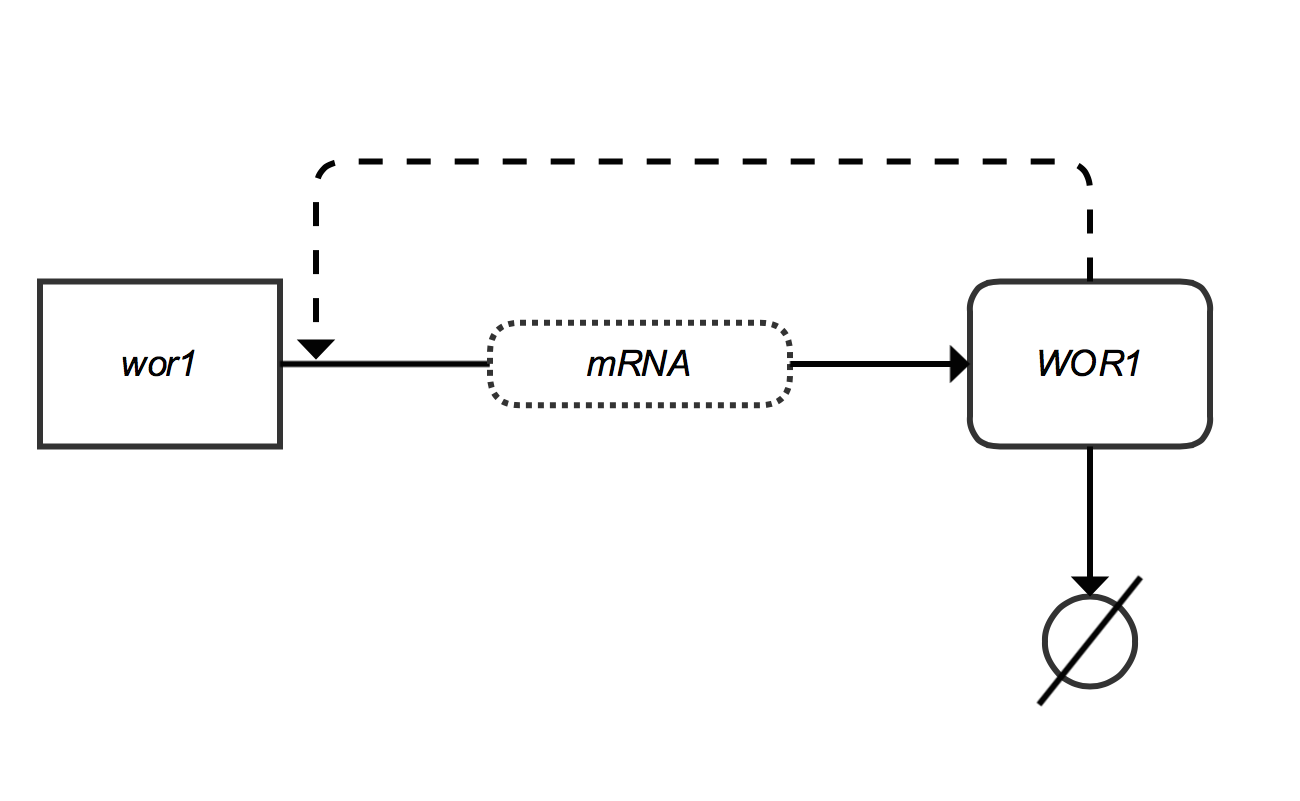
\includegraphics[width=0.6\textwidth]{./figures/singlePositive.png}
        \caption{Positive feedback system of the \textit{wor1} gene's feedback with the WOR1 protein, including mRNA and degradation of the protein.}
        \label{singlePositive}
        \end{figure}            

        \begin{figure}[h!]
        \centering
        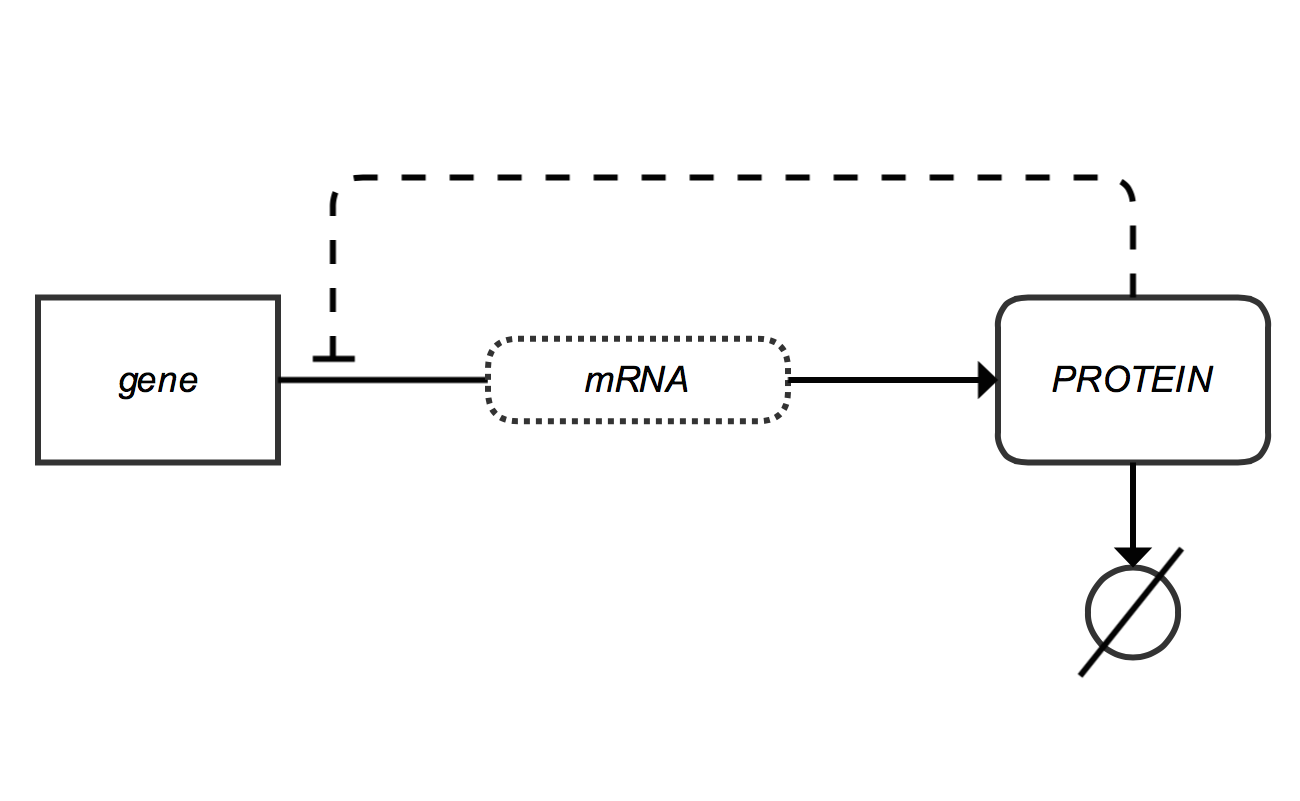
\includegraphics[width=0.6\textwidth]{./figures/singleNegative.png}
        \caption{Negative feedback system of a gene with a protein including mRNA and degradation of the protein.}
        \label{singleNegative}
        \end{figure}
        
        %@Steph do we need to change ligand%
        The approach taken to constructing a system of equations for a positive and negative feedback dynamical system was inspired by the approach of de Jong in \cite{slides}, it includes mRNA, protein and degradation. Hills equation is used to model the fraction of possible binding sites on the receptor that are occupied by a ligand. 
        
            \subsubsection{Positive Feedback} 
            Using this approach the positive feedback system depicted in Figure \ref{singlePositive} can be mathematically described by the following equations.
            
            \begin{align*}
                \frac{dx_1}{dt} &= \kappa_1 h(x_2) - \gamma_1 x_1 \\
                \frac{dx_2}{dt} &= \kappa_2x_1- \gamma_2 x_2\\
                \text{The variables are denoted as:}&\\
                x_1 &= \text{Concentration of mRNA}\\
                x_2 &= \text{Concentration of Protein}\\
                \kappa_1, \kappa_2 &= \text{Production Rate of mRNA and Protein respectively}\\
                \gamma_1, \gamma_2 &= \text{Degredation Rate of mRNA and Protein respectively}\\
                h(x) &= \frac{x^n}{k^n+x^n} \text{where $k$ describes a threshold concentration and $n$ a strength}
            \end{align*}
            
            One of these single gene positive feedback system as described above exists in Candida Albicans, for the sake of relevance we'll be discussing the above system as it pertains to this specific system where the gene is \textit{wor1} and the protein is WOR1. In order to investigate the system further the nullclines and phase portrait are plotted in Figure \ref{stabilitySinglePositive}. 
           \\
\subsubsection{Negative Feedback} 
            The same approach as used in analysing the positive feedback system was applied to modelling the negative feedback system. The only difference in the set of equations that describe the system is a modification to the Hill equation. Instead of the hill equation being $h(x) = \frac{x^n}{k^n + x^n}$ we use $h(x) = \frac{k^n}{k^n+x^n}$. This is a small modification with quite a drastic impact. Modelling the nullclines and phase portrait to investigate the behaviour of the system around its stability points in Figure \ref{stabilitySingleNegative}. 
\subsection{Multiple Gene Systems}
        A vast number of multiple gene feedback loops are possible, sadly most of these systems are out of the scope of this paper. %Tears, lots of tears.
        The two that will be investigated are mutual positive feedback between two genes and mutual negative feedback between two genes. A different approach to modelling these will be adopted as compared two the single gene cases. In order to keep things relatively manageable the impact of mRNA will be neglected and only the concentration of protein in each system will be looked at, this is the simplified approach to this problem adopted by de Jong in \cite{multiGene}. 

        \begin{figure}[h!]
        \centering
        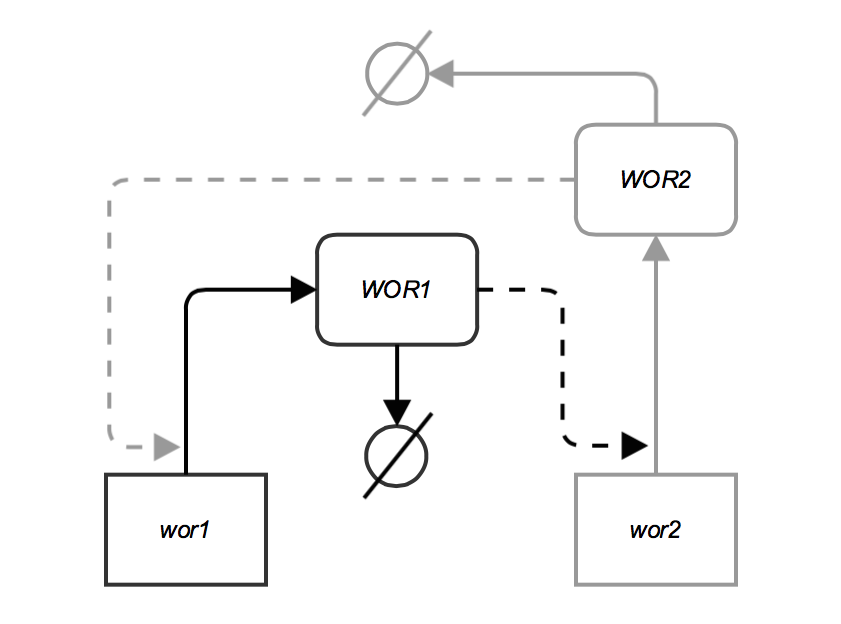
\includegraphics[width=0.6\textwidth]{./figures/doublePositive.png}
        \caption{Positive feedback system of the \textit{wor1} gene and the \textit{work2} gene whereby WOR1 promotes WOR2 and WOR 2 promotes WOR1}
        \label{doublePositive}
        \end{figure}            
    
        \begin{figure}[h!]
        \centering
        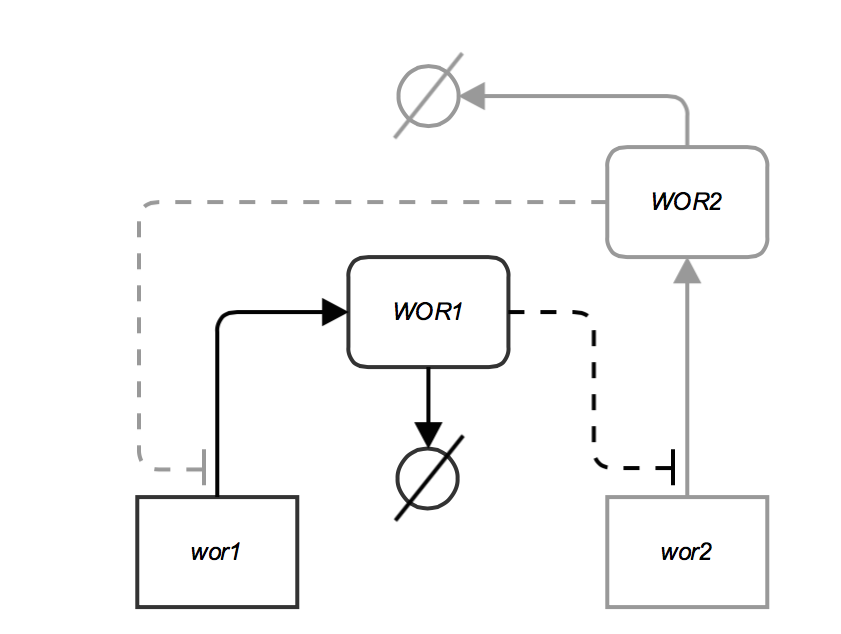
\includegraphics[width=0.6\textwidth]{./figures/doubleNegative.png}
        \caption{Negative feedback system of two genes where the protein mutually inhibit each other.}
        \label{doubleNegative}
        \end{figure}
                 
            \subsubsection{Positive Feedback}
            A network of 2 genes with mutual positive feedback also exits in the Candida Albicans cell between the \textit{wor1} \& \textit{wor2} genes, this is the system as depicted in Figure \ref{doublePositive}. The equations describing this system are given below.
            
            \begin{align*}
                \frac{dx_1}{dt} &= \kappa_1 h(x_2) - \gamma_1 x_1 \\
                \frac{dx_2}{dt} &= \kappa_2 h(x_1) - \gamma_2 x_2 \\
                \text{The variables are denoted as:}&\\
                x_1 &= \text{Concentration of WOR1}\\
                x_2 &= \text{Concentration of WOR2}\\
                \kappa_1, \kappa_2 &= \text{Production Rate of WOR1 and WOR2 respectively}\\
                \gamma_1, \gamma_2 &= \text{Degredation Rate of WOR1 and WOR2 respectively}\\
                h(x) &= \frac{x^n}{k^n+x^n} \text{where $k$ describes a threshold concentration and $n$ a strength}
            \end{align*}
            
            Again, the nullclines and phase portrait are plotted to investigate the behaviour around the stability points. This can be seen in Figure \ref{stabilityDoublePositive}.   
\\         
\subsubsection{Negative Feedback}
            Although, a known double feedback does not directly exist between two genes in Candida Albicans it is perhaps the most interesting situation to look at. The system is depicted in Figure \ref{doubleNegative}, and the equation describing it are identical to those describing the positive apart from the negative hall equation being used as described in the negative single gene model. Again, applying our standard analysis for stability of the system Figure \ref{stabilityDoubleNegative}. 
%
%\section*{Methods}
%
%We began by investigating a single gene self regulating itself in Matlab. Genes code for proteins through a chain of processes.  In the case of Candida Albicans WOR1 binds to it's own DNA regulatory region which in turn activates the production of more WOR1 creating a positive feed back loop. 
%
%A Diagram for the system is given below:\\
%
%\begin{center}
%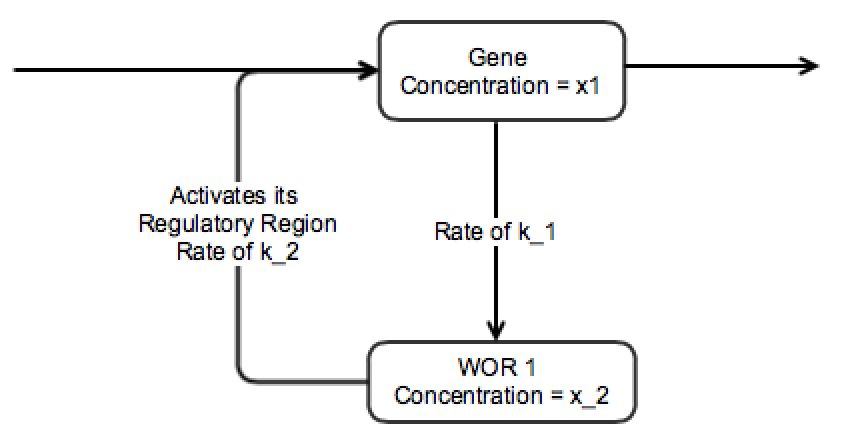
\includegraphics[scale = 0.75]{Posfeed.png}
%\end{center}
%
%The Rate of change for WOR1 is a system with an input of activation rate dependent upon the amount of $x_1$ and a output given by the degradation of itself $x_1$. The equation governing $x_1$ is a little more complex. As the activation can only occur on certain sites. The fraction of these occupied sites is given by Hill's equation \cite{Hill}. The system of equations is given below.
%
%\begin{align}
%\frac{dx_1}{dt} &= k_1\left(\frac{x_2^n}{\alpha^n + x_2^n}\right) - \gamma_1x_1\\
%\frac{dx_2}{dt} &= k_2x_1 -\gamma_2x_2
%\end{align}
%
%	%insert image of equations here
%Where:
%\begin{itemize}
%	\item $x_1 =$ mRNA concentration
%	\item $x_2 =$ protein concentration
%	\item $k(1), k(2) > 0$ production rate constants
%	\item $\gamma(1), \gamma(2) > 0$ degradation rate constants
%\end{itemize}
%
%
%This system of equations was the analysed using Matlab and it's ode45 function. The first step in analysing this system was comparing the fraction of the occupied sites against the amount of WOR1. 
%
%\begin{figure}[h]
%\caption{Model of occupied reaction sites versus concentration of WOR1}
%\centering
%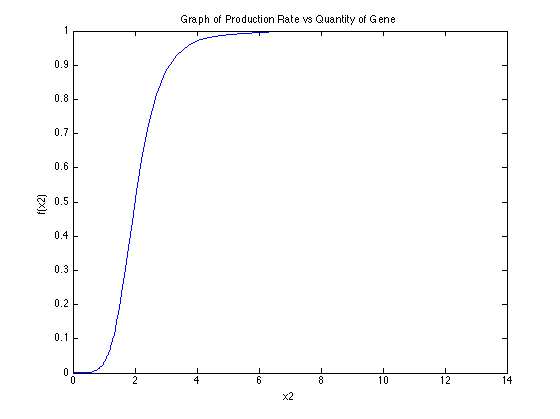
\includegraphics[scale = 0.5]{prodRateVsQuant.png}
%\label{fig:Hill}
%\end{figure}
%
%We can see from Figure \ref{fig:Hill} that there are two distinct states,  a state of no occupation and a state of complete occupation. This does not, however describe how the system behaves around these two states. To gain more insight into the behaviour of this system we modelled the nullclines as described by 
%	\begin{align}
%		\dot{x}_1=0 \Rightarrow x_1=\frac{k_1}{\gamma_1}f(x_2)\\
%		\dot{x}_2=0 \Rightarrow x_1=\frac{k_2}{\gamma_2}f(x_2)
%	\end{align}
%
%The Phase portraits around each stationary point were also modelled in Figure \ref{fig:phaseport}  to investigate the stability of each point.
%
%\begin{figure}[h]
%\caption{Nullclines for positive feedback system}
%\centering
%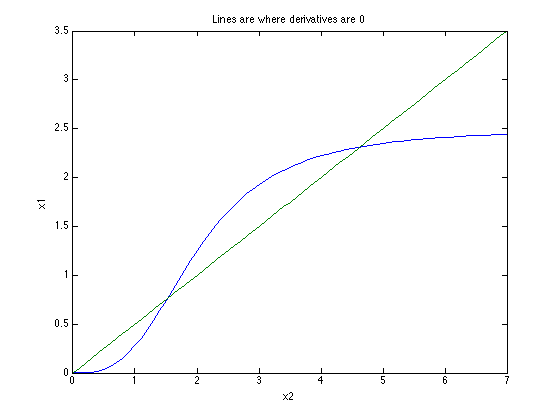
\includegraphics[scale = 0.5]{zeros.png}
%\label{fig:nullclines}
%\end{figure}
%
%\pagebreak 
%
%\begin{figure}[h]
%\caption{Phase Portraits for the three stationary points}
%\centering
%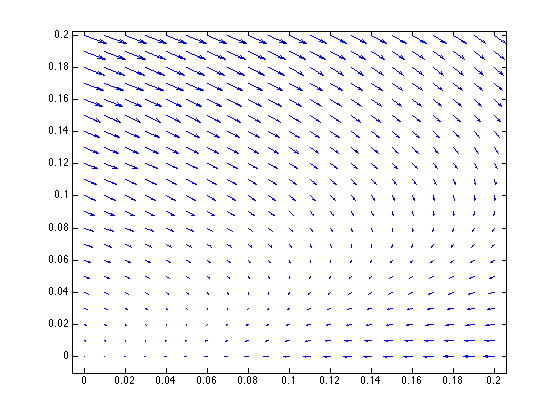
\includegraphics[width=.3\textwidth]{zerozero.png}\hfill
%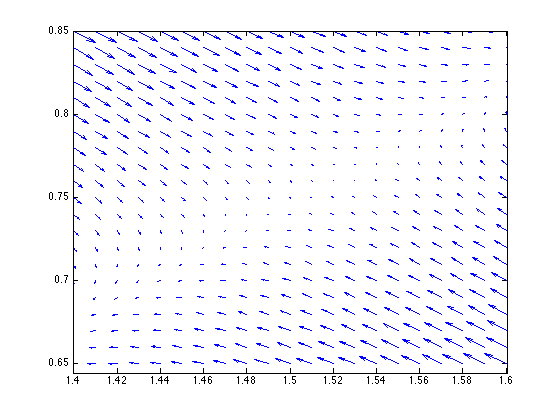
\includegraphics[width=.3\textwidth]{unstable.png}\hfill
%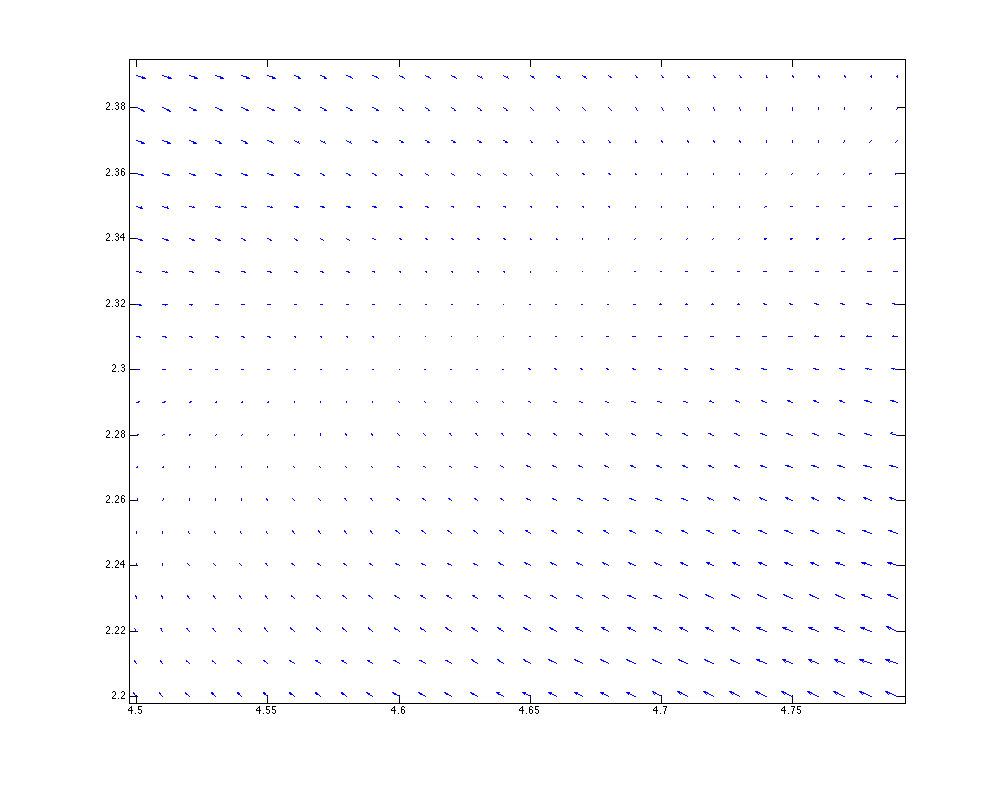
\includegraphics[width=.3\textwidth]{max.png}
%\label{fig:phaseport}
%\end{figure}
%
%Figure \ref{fig:nullclines} suggests that there are three stationary points of which the rate of change for $x_1$ or $x_2$ is zero. Further investigation using Figure \ref{fig:phaseport} reveals that the first and last points are stable but the middle point is an unstable stationary point. Thus we can conclude that this system of equation is bistable. The stability points occur when all the reaction sites are occupied or when none of them are. This models very closely the observed opaque switching behaviour of the Candida Albans in the absence of an interim stability point.\\ 
\section{Discussion}

\subsection{Findings}
Single Gene\\
\\
Positive Feedback\\ 
We can see from these that there are three stationary points in this system. The middle stationary point around $(1,1)$ is not stable and of not much practical interest as even infinitesimally small perturbations will cause it to tend towards one of the other stationary points of which are both stable. It can be concluded from this that the system is bi-stable as there are exactly two stability points. Taking this one step further the behaviour of the protein around these stability points can be investigated to get a sense of the difference in physical state of the system being at either of the stability points. 
            
             \begin{figure}[h!]
            \centering
            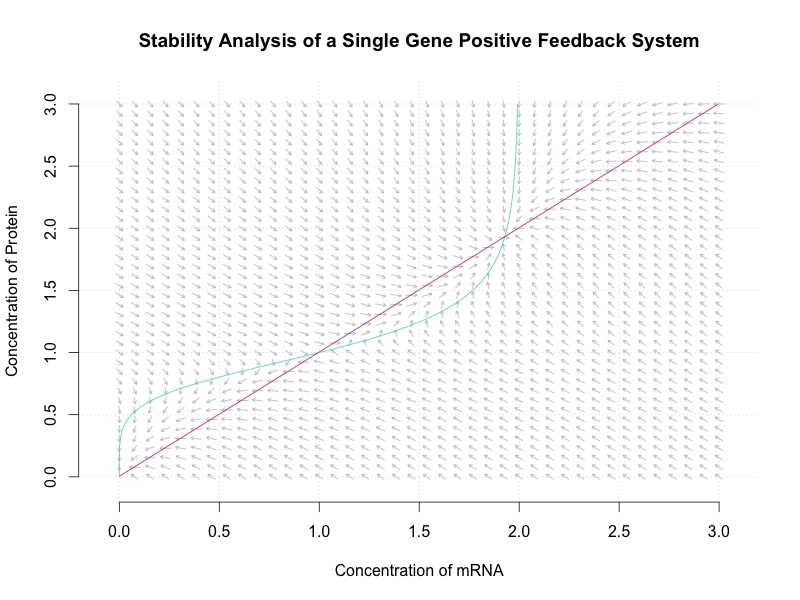
\includegraphics[width=0.6\textwidth]{./figures/stabilitySinglePositive.jpeg}
            \caption{The stability of stationary point present in a single gene positive feedback system. The red line represents the nullcline for the protein and blue the nullcline of mRNA. The arrows represent the direction of change for the system at a given state.}
            \label{stabilitySinglePositive}
            \end{figure}
            
                    
             \begin{figure}[h!]
            \centering
            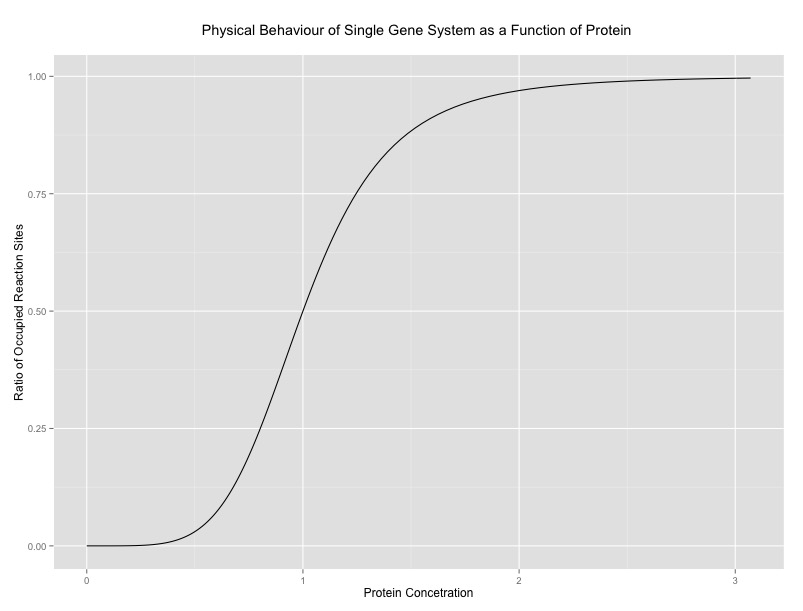
\includegraphics[width=0.6\textwidth]{./figures/singlePositiveHill.jpeg}
            \caption{Compares the fraction of occupiable receptor sites on the protein that are currently occupied against the concentration of protein.}
            \label{singlePositiveHill}
            \end{figure}
    
            The fraction of available binding sites on the receptor was modelled against the concentration of protein in Figure \ref{singlePositiveHill}. This shows that as the concentration of protein increases the ratio of occupied receptor sites increases until all sites are occupied. We can think of this as a state where %%@Steph what does having a heap of protein mean? 
            White is dominant and Opaque is subdued %%This is completele ramble DO NOT INCLUDE IN FINAL WITHOUT CHECKING %%"To switch to the opaque state, Wor1p expression must increase until it reaches a critical threshold level at which point stable Wor1p expression is maintained by positive feedback on its own promoter."
\\
Negative Feedback\\
We can see that the negative feedback system has only one stationary point which is in turn its only stability point. It appears that the negative feedback system of a single gene is incapable of producing a bistable or multi stable state.  
            \begin{figure}[h!]
            \centering
            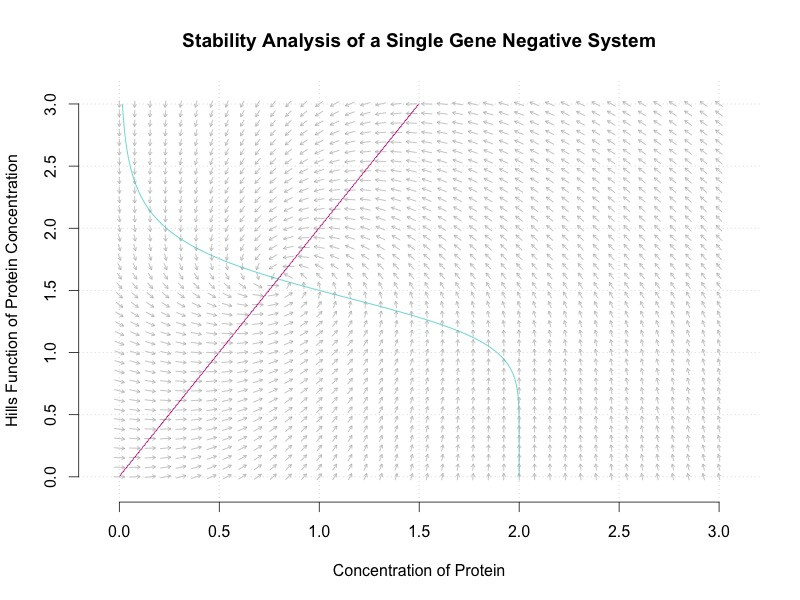
\includegraphics[width=0.6\textwidth]{./figures/stabilitySingleNegative.jpeg}
            \caption{The stability of stationary point present in a single gene negative feedback system. The red line represents the nullcline for the protein and blue the nullcline of mRNA. The arrows represent the direction of change for the system at a given state.}
            \label{stabilitySingleNegative}
            \end{figure}
Multiple Gene System\\
\\
Mutual Positive Feedback\\
 This system behaves somewhat similar to the single gene positive feedbacks system, similarly it has three stationary points, two of which are stable and one of  which is unstable. This makes sense when considering the behaviour of the general system %% Bullshiting need to elaborate            
            \begin{figure}[h!]
            \centering
            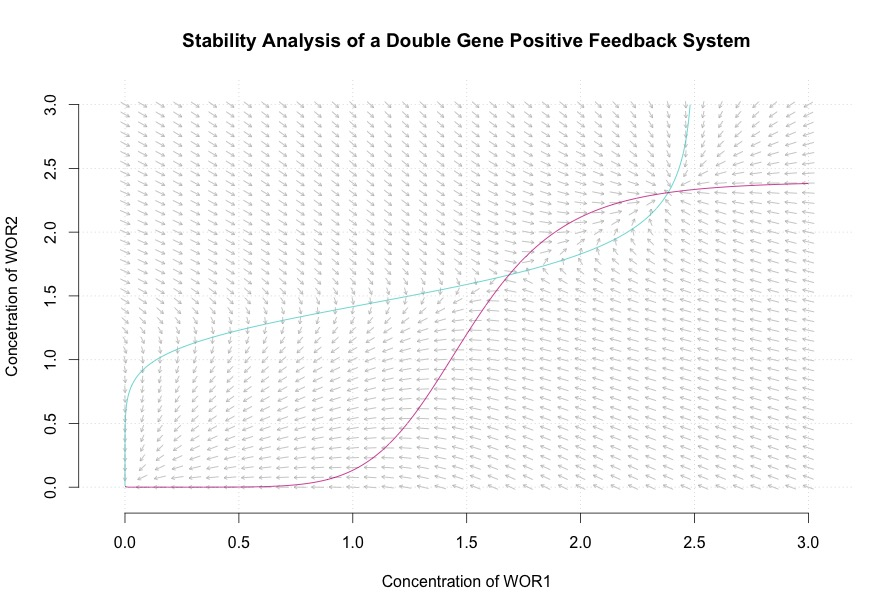
\includegraphics[width=0.6\textwidth]{./figures/stabilityDoublePositive.jpeg}
            \caption{The stability of stationary point present in a double gene positive feedback system. The red line represents the nullcline for the protein and blue the nullcline of mRNA. The arrows represent the direction of change for the system at a given state.}
            \label{stabilityDoublePositive}
            \end{figure}
Mutual Negative Feedback\\
We see something completely different to the single gene case. Whereas the single gene with negative feedback only produce a single stationary and stability point the double gene with mutual negative feedback generates three stationary point with two of them being stable. This demonstrates that you can generate a bistable system out of solely negative feedback. An indirect double negative feedback system exists in Candida Albicans but requires the modelling of an additional gene which is beyond the scope of this paper.         
            \begin{figure}[h!]
            \centering
            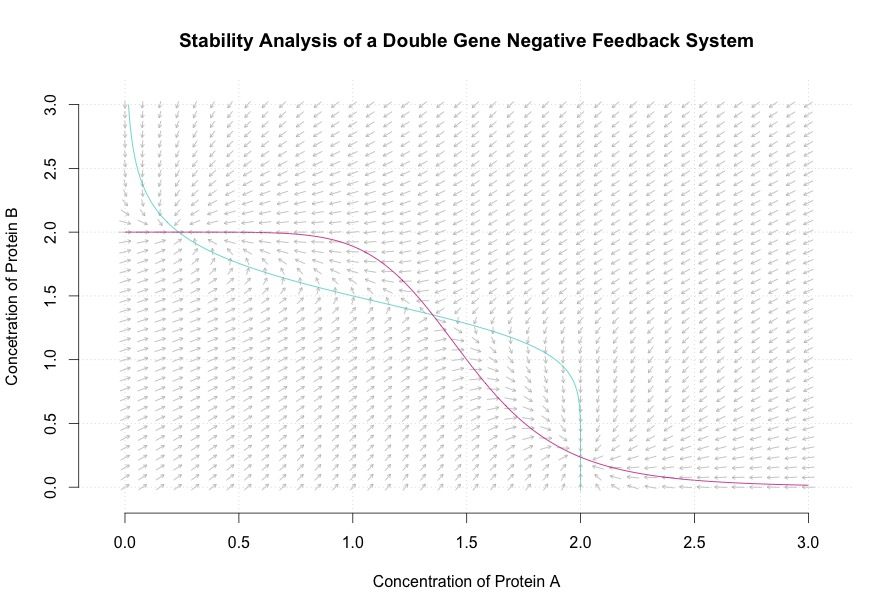
\includegraphics[width=0.6\textwidth]{./figures/stabilityDoubleNegative.jpeg}
            \caption{The stability of stationary point present in a double gene negative feedback system. The red line represents the nullcline for the protein and blue the nullcline of mRNA. Thwidth=0.6e arrows represent the direction of change for the system at a given state.}
            \label{stabilityDoubleNegative}
            \end{figure}
\\
\subsection{Comparison of Methods}
There are other many possible ways of mathematically modelling gene regulation using differing methods. Here we will compare and contrast our method to evaluate its value.
\\
Our chosen method was solving differential equations. Differential equations are a power method of simulating gene regulation due to the many known methods for solving and computing them. Matlab come with packages that solve differential equations for the user, instead of having to specifically code these yourself. There also exist many well known methods of analysing differential equations and understanding their results. This was particularly beneficial, allowing us to understand how the system was behaving based on which set of genes, proteins and feedbacks that were being modelled.
\\
Some downsides of using our method was that we did not know appropriate values of parameters to accurately simulate the real system. An assumption of differential equations is that you are working with continuous variables. On the molecular level this is not true, you can't have half a protein or a gene. For this reason it would be far more realistic to use a stochastic model. 
\\
Stochastic models are used to describe systems of random variables and their time evolution.  Stochastic processes are the counterpart to a deterministic system. As previously mentioned before, a stochastic method is a better reflection of the discrete nature of gene regulation than continuous variables. By using a continuous model we have made an assumption about the nature of the system that may inaccurately represent its time evolution.
\\
Using a stochastic method also has its own issues and raises many questions. For example,the WOR1 auto regulatory feedback loop is known to cause a stochastic W/O transition. However, this contradicts the experimental fact that the WOR2? produces a stable white form.  This indicates that there exists an unknown negative regulation that generates a positive feedback loop between WOR1 and EFG1. This may only be possible if the unknown protein competes with the regulation of wor1 gene that keeps the system in the default state. (https://lifeware.inria.fr/~soliman/publi/KSF09jtb.pdf page 6)
\\
This tells us that modelling using stochastic methods is not some kind of magic bullet. Using stochastic methods still leads to major differences between experimental observation and reality.

\subsection{Expanding the Model}

Many environmental factors are known to effect the frequency of opaque-white switching such as temperature and CO2 concentrations. 
\\
(Huang, Guanghua et al. ?CO2 Regulates White-Opaque Switching in Candida Albicans.) demonstrated that a temperature shift from 25-37 degrees caused an increase in the O/W switching rate. This temperature increase also lead to a total increase in production of both opaque and white states.
Studies of the effect of CO2 concentration on the the switching states (Huang, Guanghua et al.) showed that W/O was stimulated and O/W was blocked. They analysed the induction of switching by CO2 in \textit{wor1} discovering that it suppressed switching of white cells.
\\
Our model has not taken temperature or CO2 concentration into account which, as described above, would impact the production and degradation rates significantly. The model is theoretical and does not represent realistic values for concentrations of proteins, instead modelling the generalised behaviour of its feedbacks.To accurately apply our model to reality we need to introduce many dependancies on environmental conditions to our constants. Modelling this dependancy exceeds the scope of this assignment and requires significant research and data.
\\
%[Steph's mumbo jumbo... in progress... cite, check italics/capitalisation]
For any given gene, there may be any number of transcription factors which regulate its expression. For C. albicans, Wor1 and Wor2 are not the only transcription factors which regulate white-opaque switching. Transcriptional factors Efg1 and Czf1 also have regulatory roles. They too are involved in a network of positive and negative feedback loops (STEPH TO CITE 1) which are not accounted for in our model. Czf1, similar to Wor1 and Wor2, promotes the opaque state, whilst its absence supports the cell?s white state (STEPH TO CITE 1). The reason being that Czf1 represses the expression of transcription factor Efg1, which stimulates the cell?s white state (STEPH TO CITE 1).
\\
Other non-coding intracellular molecules further complicate gene regulatory models such as ours. Although our model disregards these molecules, some, such as small interfering RNA (siRNA) and microRNA (miRNA) have been shown to have a profound affect on gene regulation (STEPH TO CITE). In C. albicans,  siRNA and miRNA regulate gene expression by silencing genes such as Wor1 at a post-transcriptional level. miRNA bind to mRNA to repress translation/induce gene silencing. Whether this process occurs due to mRNA degradation or translational inhibition is heavily contested (STEPH TO CITE). Unlike most other processes involving mRNA, miRNA only require partial complementary base pairing. Since they lack specificity, an individual miRNA may target many different mRNA strands. Therefore the up regulation and down regulation of a single miRNA can effect multiple networks.
%[1+1 = 2 ...just checking I'm still sane... ]
\\
Our current model also assumes a system of gene expression which is not susceptible to mutations. However, the effect of genetic mutations such as the deletion of mediators (coactivators of transcription) have been shown to affect the expression of white and opaque states. For example, the deletion of med3, destabilises the opaque state, whereas the deletion of med12 coincides with a 93% (CITE 2) opaque-to-white switching frequency. HOW DO I MAKE THE PERCENTAGE IN THE LINE ABOVE BLACK SO IT APPEARS IN THE REPORT...btw do I need to use less bio jargon?
%%blah 
The factors discussed above are by no means a comprehensive account of all the factors which may influence this dynamical system.  %%insert some vague bullshit about how much more complex these systems are on a biological level. end section.
\\
\section{Model evaluation and conclusion}
Our model does provide insight into the way a system of genes may regulate itself. However it uses a large number of assumptions in order to reach its result. Due to this it is very difficult to judge whether our model accurately represents the regulation of \textit{wor1} and \textit{wor2} in a real biological system.
\\
We have demonstrated possible behaviours of the system under certain condition, but also explored how other variables or methods of modelling may cause the real system to differ from our results. We have explored and discussed a number of methods used in modern mathematical modelling.
\\
It is clear that mathematical models are a powerful technique for analysing biological systems. In future years it is likely that collaboration between scientists and mathematicians will lead to deep and accurate insights into the way these systems behave.

\bibliographystyle{unsrt}


\bibliography{Bibliography}
http://www-sop.inria.fr/comore/arcgdyn/28fev/arc03-intro.pdf

M. P. kolotila, R. D. Diamond (1990) Effects of neutrophils and invitro oxidants on the survival and phenotypic switching of Candida albicans WO-1, Infect. Immun, 58, 1174-1179.

Huang, Guanghua et al. ?CO2 Regulates White-Opaque Switching in Candida Albicans.? Current biology?: CB 19.4 (2009): 330?334. PMC. Web. 5 May 2015.
\end{document}